In this paper, we explore the connections between fixation prediction and salient object segmentation by providing a new dataset with both fixations and salient object annotations. We conduct extensive experiments on the dataset for both tasks and compare the results with major benchmarks. Our analysis suggests that the definition of a salient object is highly consistent among human subjects. We also point out significant dataset design bias in major salient object benchmarks. The bias is largely due to deliberately emphasising the concept of saliency. We argue that the problem of salient object segmentation should move beyond the textbook examples of visual saliency. A possible new direction is to look into the strong correlation between fixations and salient objects. Built on top of this connection, we propose a new salient object segmentation algorithm. Our method decouple the problem into a segment generation process, followed a saliency scoring mechanism using fixation prediction. This simple model outperforms state-of-the-art salient object segmentation algorithms on all major datasets. Our dataset together with our method provide a new insight to the challenging problems of both fixation prediction and salient object segmentation.


\begin{figure*}[p]
\centering
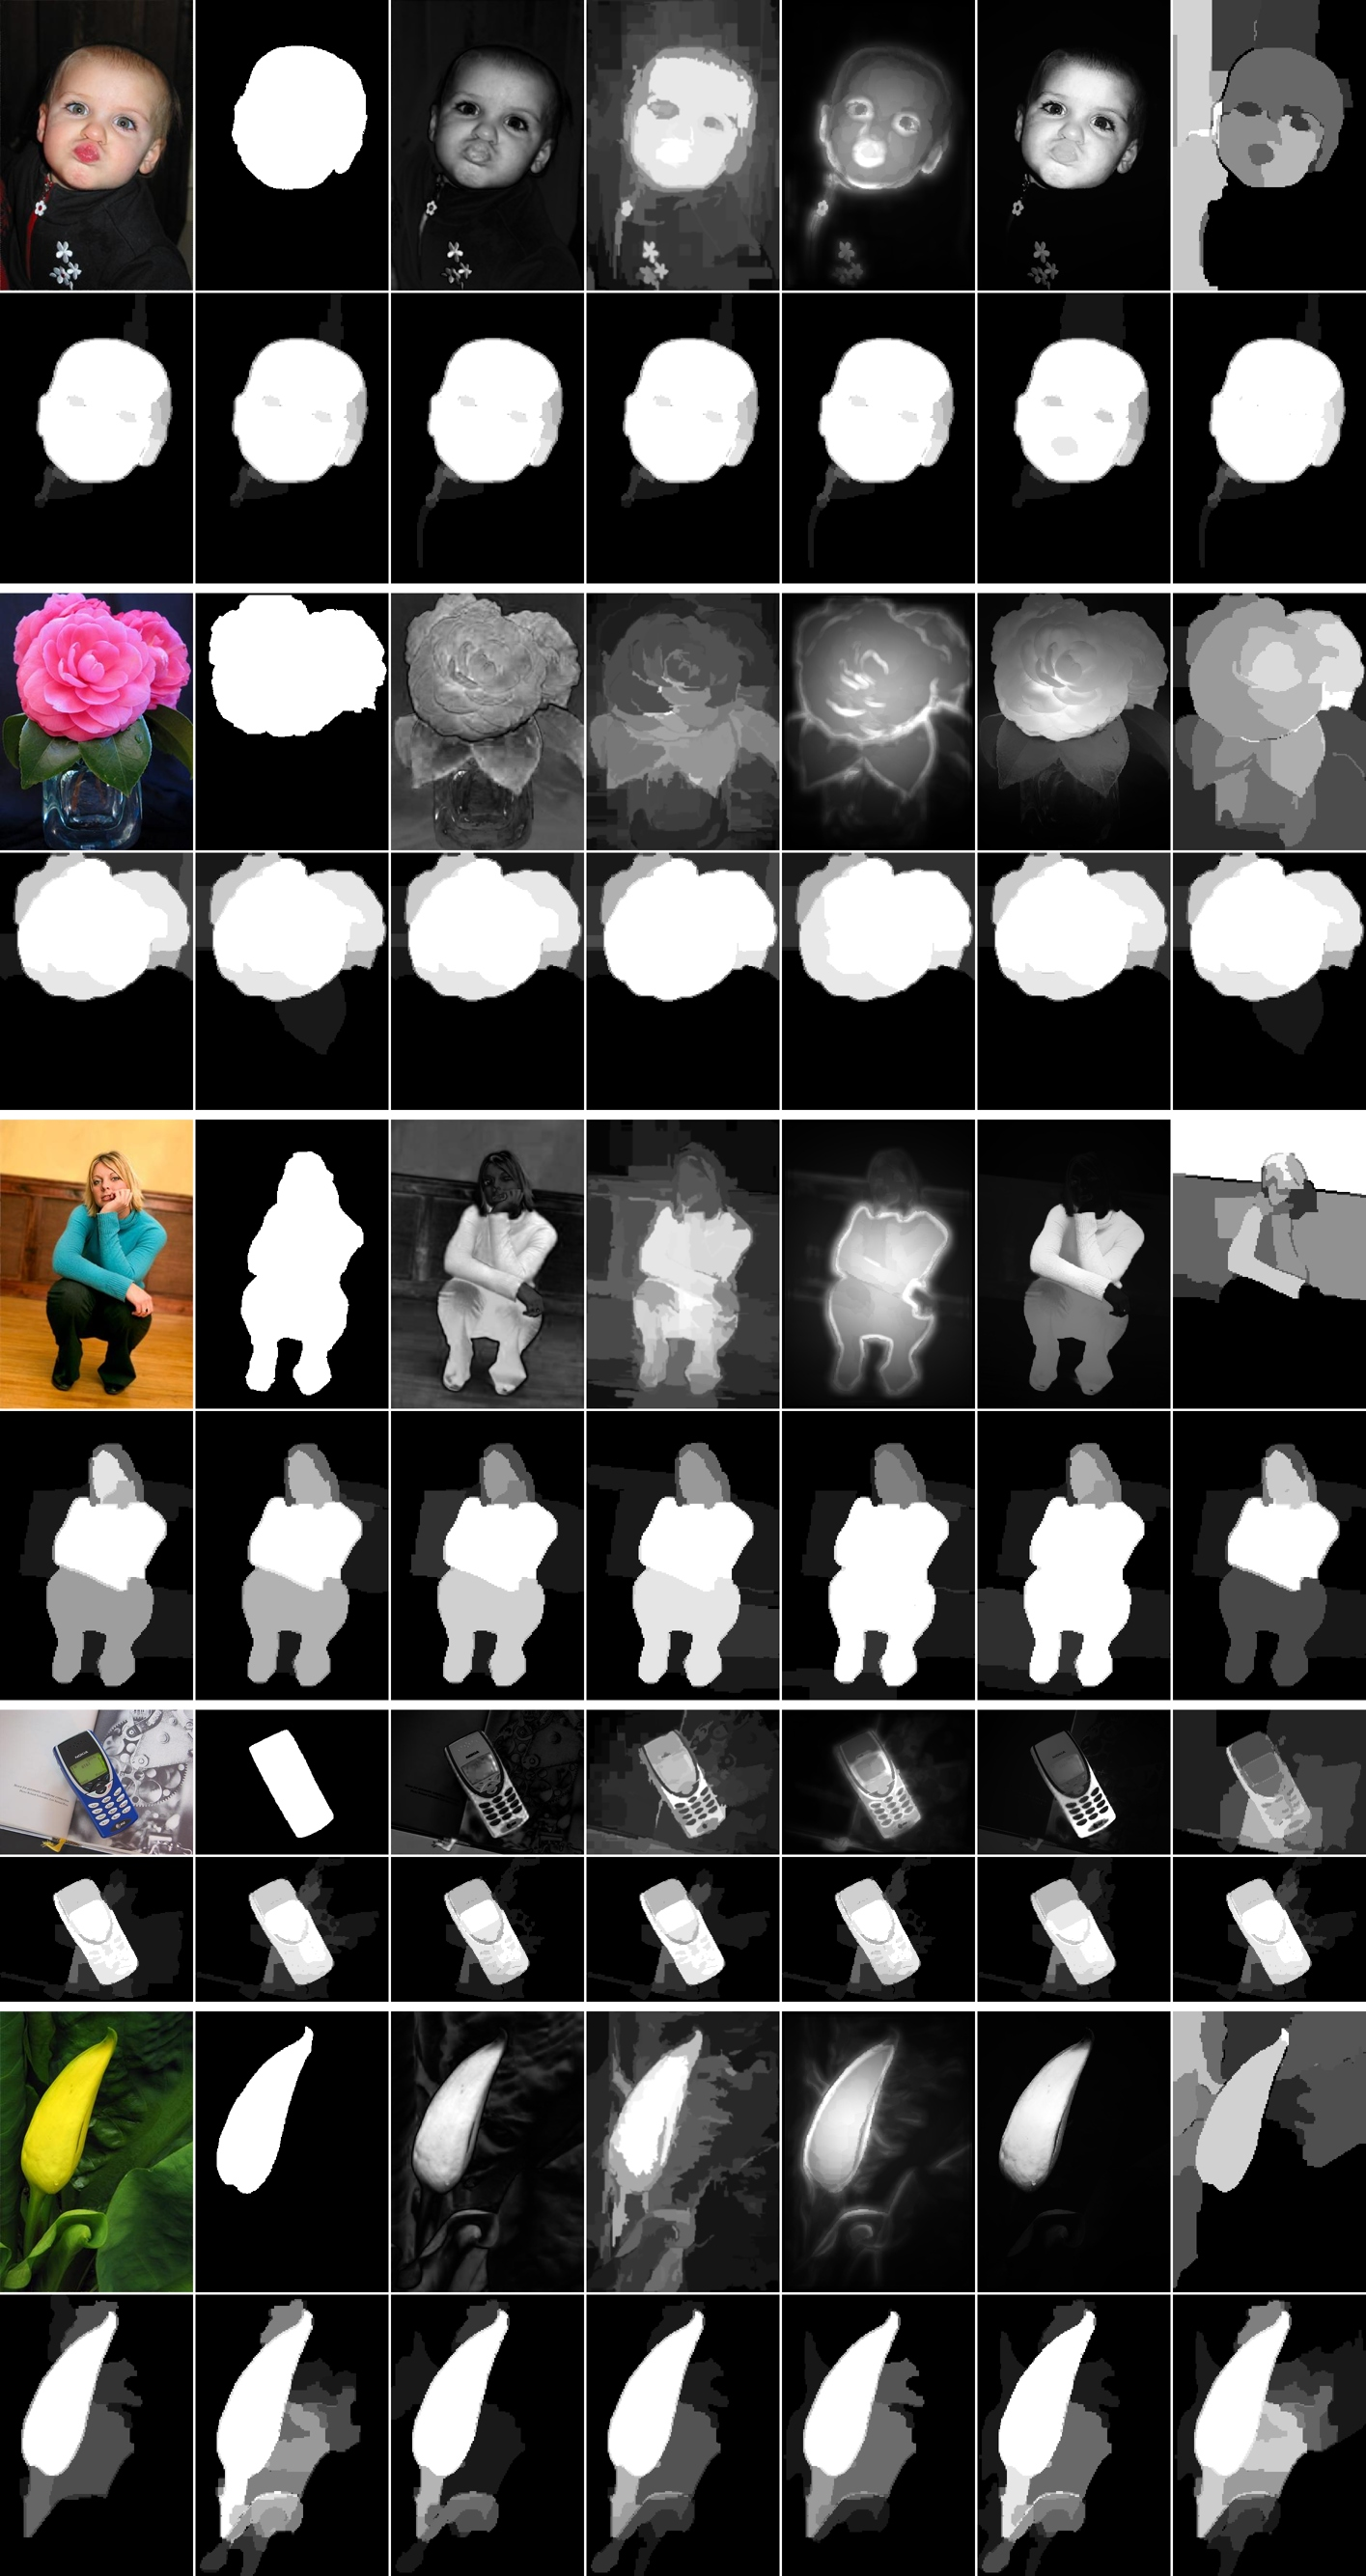
\includegraphics[width=0.65\linewidth]{ft_final.jpg}\\
\caption{Visualization of salient object segmentation results on FT. Each two-row compares the results of one image.  The first row includes results from existing methods (Left to Right): Original image, Ground-truth mask, FT, GC, PCAS, SF and CPMC ranking; The second row shows results of our method using different fixations (Left to Right): AIM, AWS, DVA, GBVS, ITTI, SIG and SUN. We are not able to report results using human fixations. The images are selected by sorting the F-measure of our results in a decreasing order. }\label{fig:ftRes}
\end{figure*}


\begin{figure*}[p]
\centering
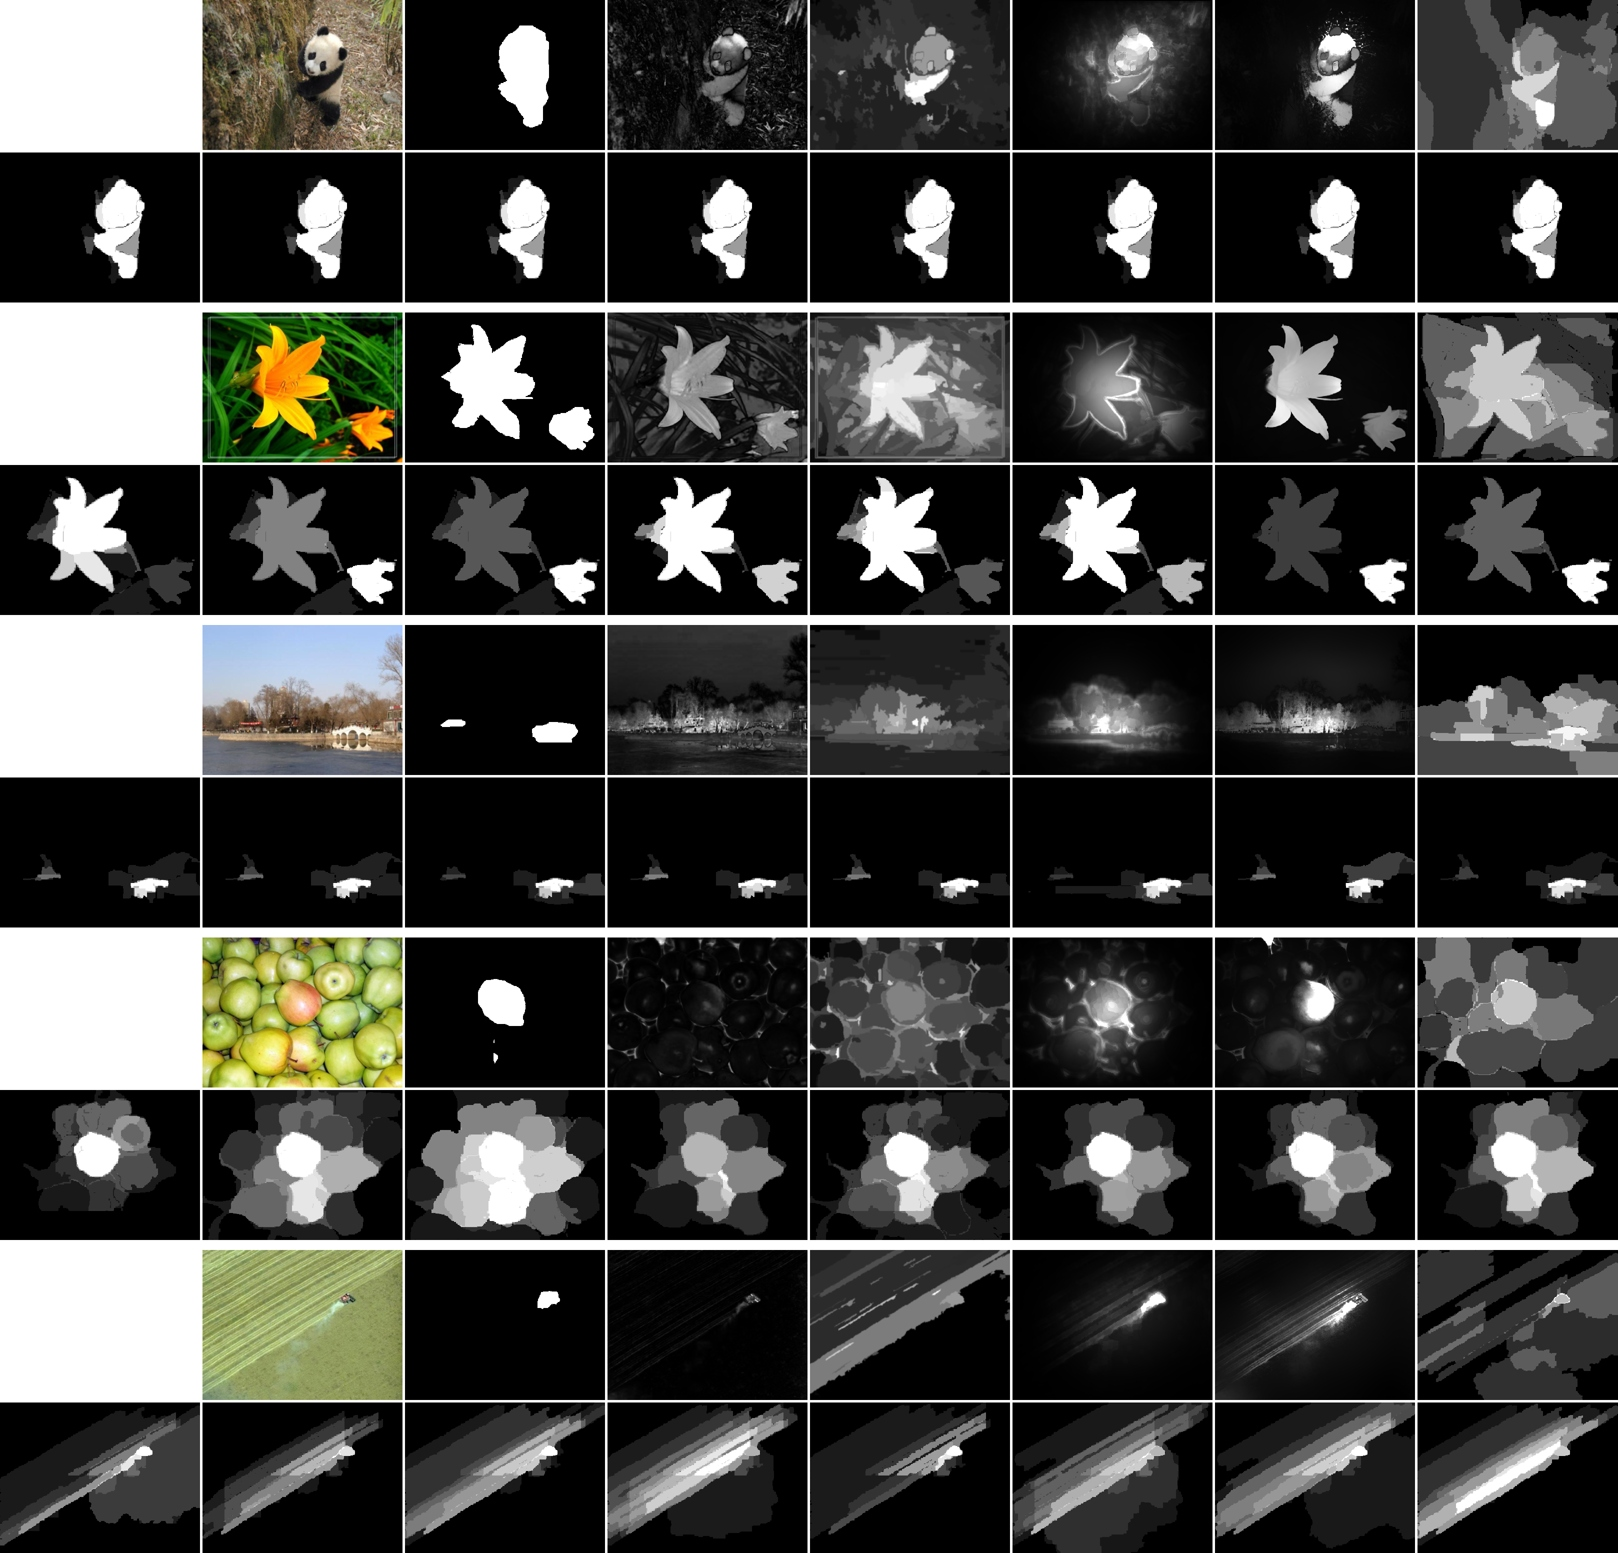
\includegraphics[width=\linewidth]{imgsal_final.jpg}\\
\caption{Visualization of salient object segmentation results on IS. Each two-row compares the results of one image.  The first row includes results from existing methods (Left to Right): Original image, Ground-truth mask, FT, GC, PCAS, SF and CPMC ranking; The second row shows results of our method using different fixations (Left to Right): Human Fixation, AIM, AWS, DVA, GBVS, ITTI, SIG and SUN. The images are selected by sorting the F-measure of our results in a decreasing order. We notice that IS favors sparse saliency maps, since it contains a significant portion of small salient objects.}\label{fig:isRes}
\end{figure*}

\begin{figure*}[p]
\centering
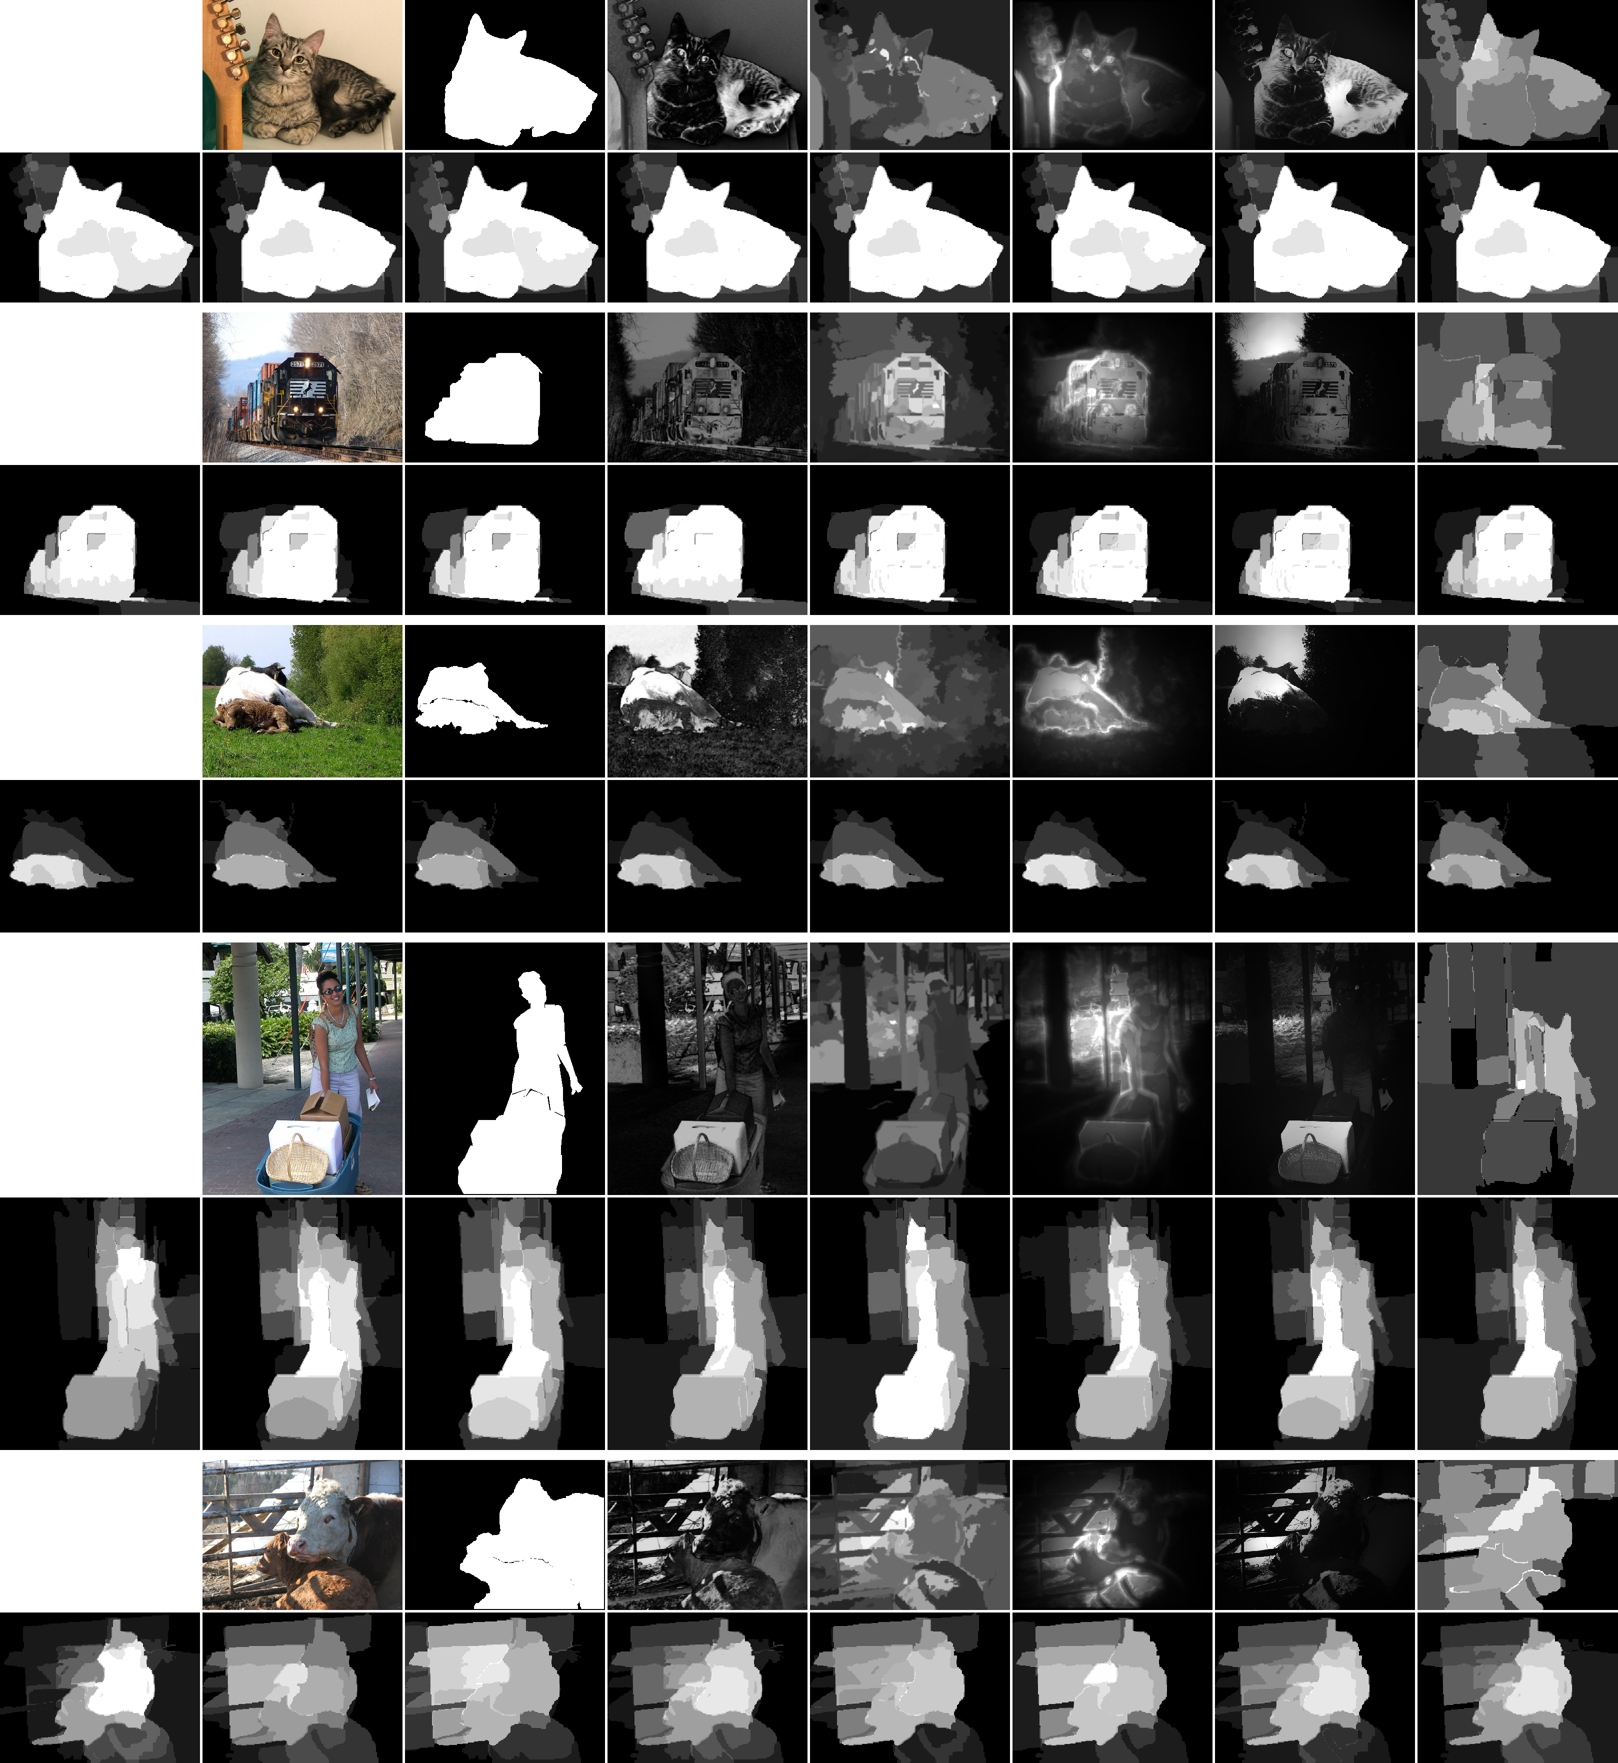
\includegraphics[width=\linewidth]{pascal_final.jpg}\\
\caption{Visualization of salient object segmentation results on PARSCAL-S. Each two-row compares the results of one image.  The first row includes results from existing methods (Left to Right): Original image, Ground-truth mask, FT, GC, PCAS, SF and CPMC ranking; The second row shows results of our method using different fixations (Left to Right): Human Fixation, AIM, AWS, DVA, GBVS, ITTI, SIG and SUN. The images are selected by sorting the F-measure of our results in a decreasing order.}\label{fig:pascalRes}
\end{figure*}

\clearpage

